\section{GRASP}
The purpose of this experiment
is to assess the behavior of the three greedy functions
used by the greedy randomized construction
of the diversification generator method,
as well as the GRASP quality threshold parameter $\alpha$.
To this end
we ran the heuristic consisting of
the construction phase only.
%(that is outside of the Scatter Search -
%Path Relinking method).
%The results are shown in table \ref{tab:}.

Several instances were tested
with different $\alpha$ values
(from 0 to 1 in steps of 0.05)
to determine the value of $\alpha$ to use.
The value of $\alpha = 0$ means that
the procedure becomes completely greedy,
and a value of $\alpha = 1$ means that
the procedure becomes completely random.
\begin{figure}[!ht]
  \centering
  \label{fig:grasp-results}
  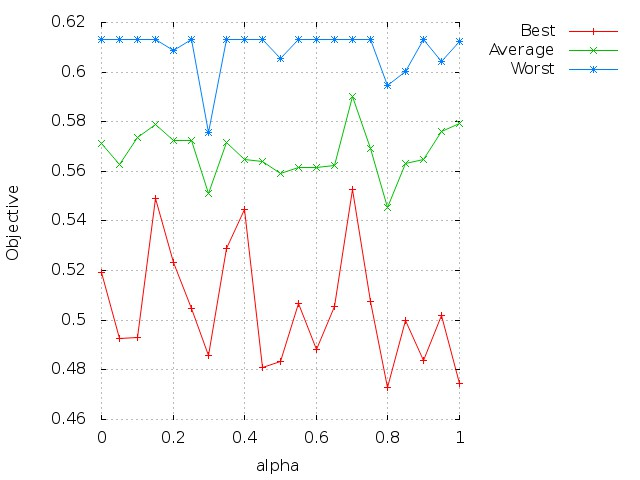
\includegraphics[scale=0.7]{GRASPr1}
  \caption{Objective value versus $\alpha$ for first greedy function}
\end{figure}
The test suggest
(see Figure \ref{fig:grasp-results})
that
with a more random version
there are more different solutions
and a wide range of objective values
achieving better solutions.
The same goes for the other functions.
%\todo{Agregar mas comentarios}
This indicates
that there is too much interaction between servers
making it difficult to attack the problem
in the construction stage.
